\begin{figure}[h]
    \centering
    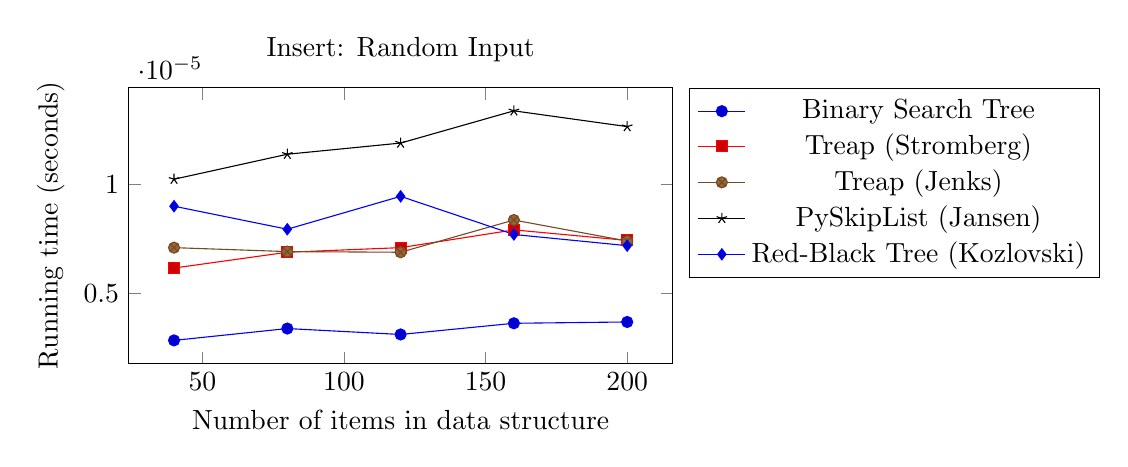
\begin{tikzpicture}
        \begin{axis}[
            xlabel={Number of items in data structure},
            ylabel={Running time (seconds)},
            title={Insert: Random Input},
            width=0.7\textwidth,
            height=2in,
            legend pos=outer north east
        ]
		\addplot coordinates {
			(40, 2.8611656991408976e-06)
			(80, 3.403281305293913e-06)
			(120, 3.1322235022174107e-06)
			(160, 3.644221574695245e-06)
			(200, 3.704456642045586e-06)
		};
		\addplot coordinates {
			(40, 6.174094403409288e-06)
			(80, 6.896915211613338e-06)
			(120, 7.10773794733951e-06)
			(160, 7.920911356569006e-06)
			(200, 7.439030817766365e-06)
		};
		\addplot coordinates {
			(40, 7.1077379473394665e-06)
			(80, 6.927032745288487e-06)
			(120, 6.896915211613251e-06)
			(160, 8.3726743616965e-06)
			(200, 7.408913284091302e-06)
		};
		\addplot coordinates {
			(40, 1.023996144955703e-05)
			(80, 1.1384427729213207e-05)
			(120, 1.1896425801691084e-05)
			(160, 1.3372184951774245e-05)
			(200, 1.2649364143570326e-05)
		};
		\addplot coordinates {
			(40, 9.005142568875059e-06)
			(80, 7.951028890244156e-06)
			(120, 9.456905574002639e-06)
			(160, 7.710088620842965e-06)
			(200, 7.198090548364913e-06)
		};
        \legend{Binary Search Tree, Treap (Stromberg), Treap (Jenks), PySkipList (Jansen), Red-Black Tree (Kozlovski)}
        \end{axis}
    \end{tikzpicture}
    \caption{Average of 10 operations, benchmarked every 40, starting at 40.}
\end{figure}